\chapter{Accueil extrascolaire}
\section{Gestion de vos lieux d'accueil extrascolaire}
Accédez à la gestion de vos lieux AES, en développant dans le volet de navigation (à gauche de l'écran) le volet \ovalbox{Accueil extrascolaire}, puis en cliquant sur l'entrée \ovalbox{Lieux} (fig. \ref{fig:aes_lieux}).

L'ensemble de vos lieux agréés est listé. Vous pouvez trier le tableau en cliquant sur les titres des colonnes. En cliquant sur "localité" par exemple, vous les trierez par ordre A-Z. 

\begin{figure}[htbp]
    \centering
    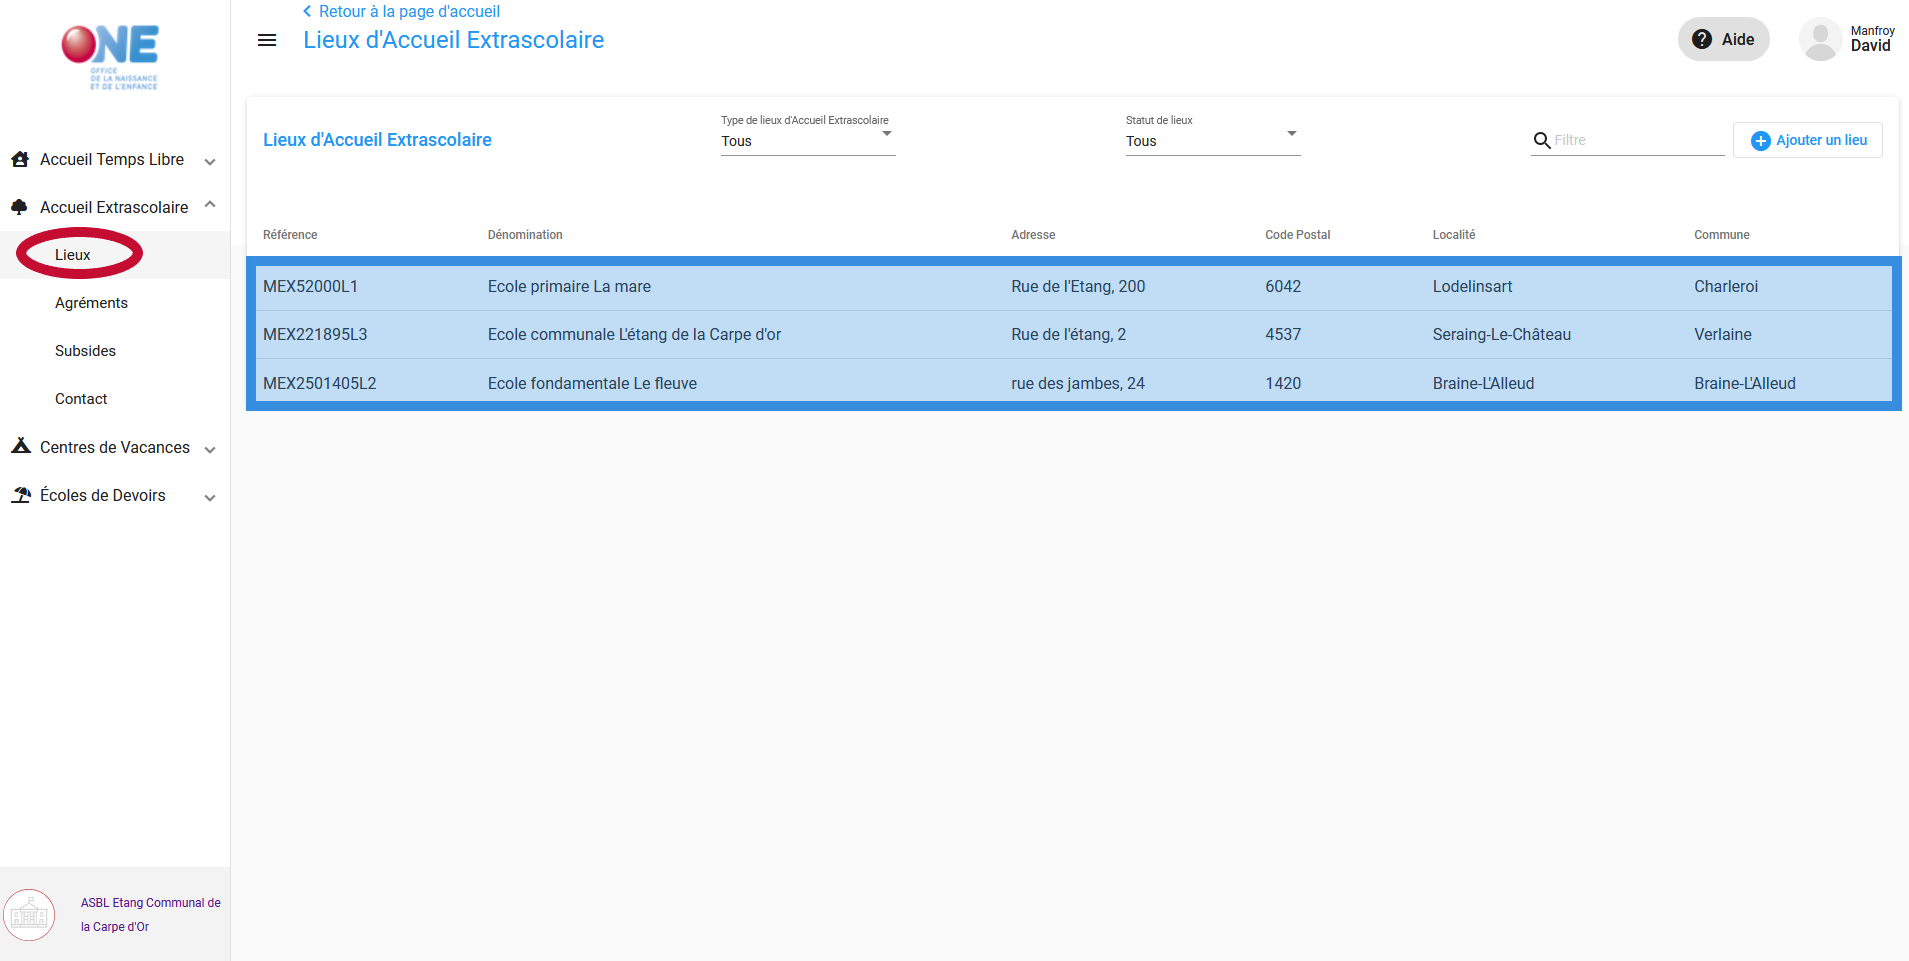
\includegraphics[width=15cm]{Images/aes/lieux.png}
    \caption{Entrée "Lieux" du volet Accueil extrascolaire: liste de vos lieux AES agrées}
    \label{fig:aes_lieux}
\end{figure}


\subsection{L'onglet lieu: informations de base du lieu AES}\label{ssec:aes_lieu}
L'onglet \ovalbox{lieu} présente plusieurs cadres d'information: 
\begin{itemize}
    \item \textbf{Lieu}: La dénomination, l'adresse et la référence MEX de votre lieu d'accueil. Si les données ne sont pas correctes, prenez contact avec votre gestionnaire de dossier de l'ONE. 
    \item \textbf{Caractéristiques}: informations concernant le type d'accueil. Vous pouvez spécifiez le type d'accueil en cliquant sur le crayon de modification. La configuration du type d'accueil conditionne l'encodage au niveau des présences. Si la case n'est pas cochées, vous ne pourrez pas renseigner ni les fréquentations d'enfants, ni les présences de l'onglet Présences. 
    \item \textbf{Agrément}: informations concernant les dates d'agrément, le type d'accueil et les journées agréées. 
    \item \textbf{Responsable de projet}: la personne de référence de votre lieu d'accueil. Vous avez la possibilité de mettre à jour la personne de contact de ce lieu d'accueil (en \textcolor{orange}{orange} dans la fig. \ref{fig:aes_lieu})
\end{itemize}

\begin{figure}[h!]
    \centering
    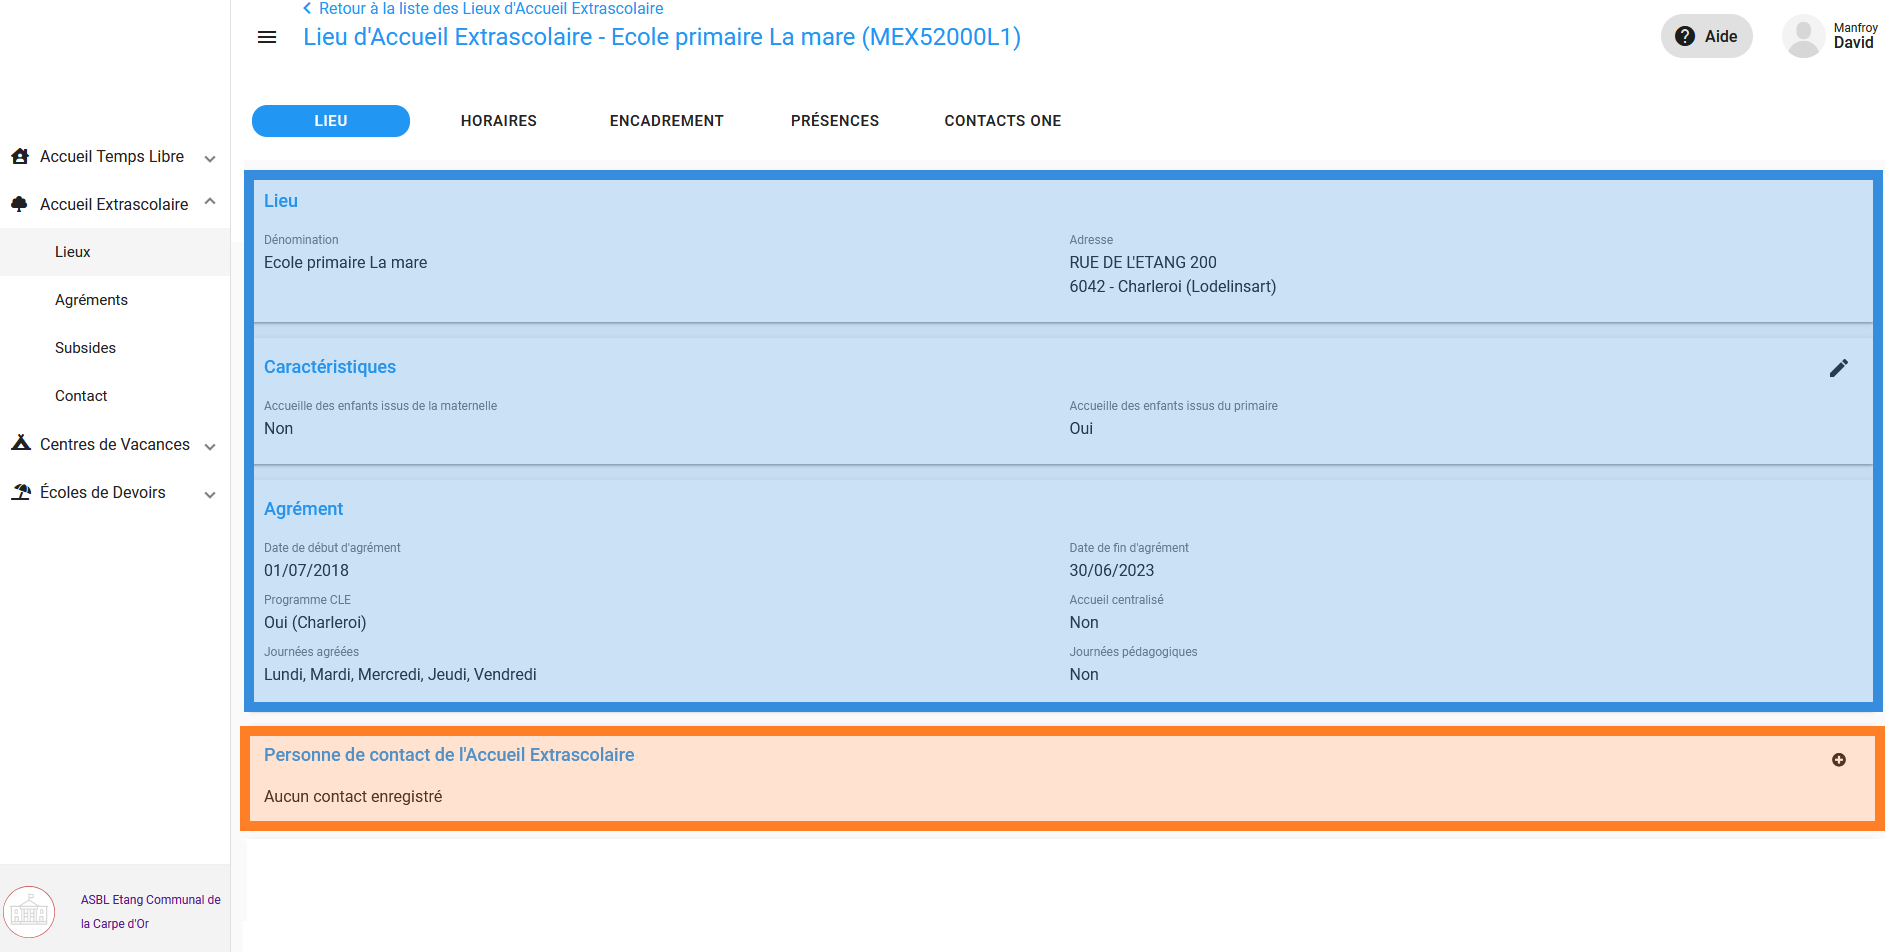
\includegraphics[width=15cm]{Images/aes/lieu.png}
    \caption{Onglet lieu: information sur votre lieu d'accueil et sur la personne de contact (responsable de projet et/ou contact administratif).}
    \label{fig:aes_lieu}
\end{figure}




\subsection{L'onglet horaire: informations sur les heures d'ouverture en période scolaire}    \label{subsec:aes_horaire}
Renseignez vos heures d'ouvertures de votre lieu d'accueil, pour l'année scolaire indiquée. Cliquez sur le petit crayon de modification pour encoder et mettre à jour les informations (en \textcolor{rouge}{rouge}, fig. \ref{fig:aes_horaires}). Encodez un commentaire éventuel (en \textcolor{bleu}{bleu}). Renseignez ensuite vos heures d'ouverture du matin et de l'après-midi (en \textcolor{orange}{orange}). N'oubliez pas d'enregistrer vos modifications en cliquant sur \ovalbox{Valider}. 

\begin{figure}[h!]
    \centering
    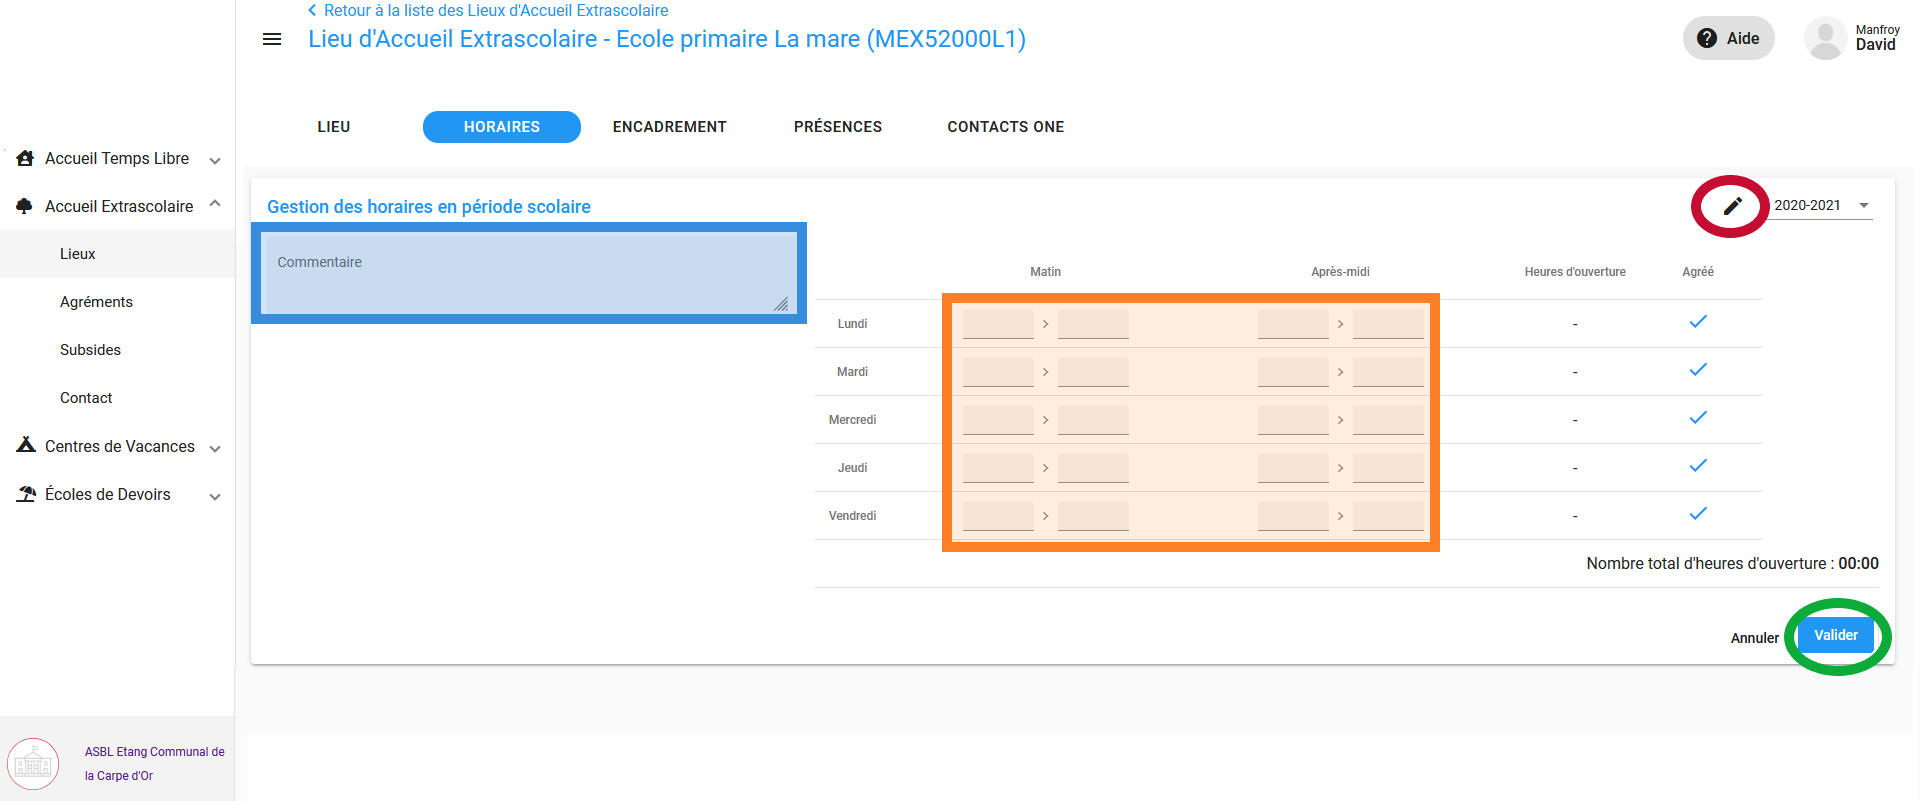
\includegraphics[width=15cm]{Images/aes/horaire2.png}
    \caption{Onglet horaires: information sur votre l'horaire de votre lieu d'accueil en période scolaire.}
    \label{fig:aes_horaires}
\end{figure}

%ancienne image de l'horaire
%\centerline{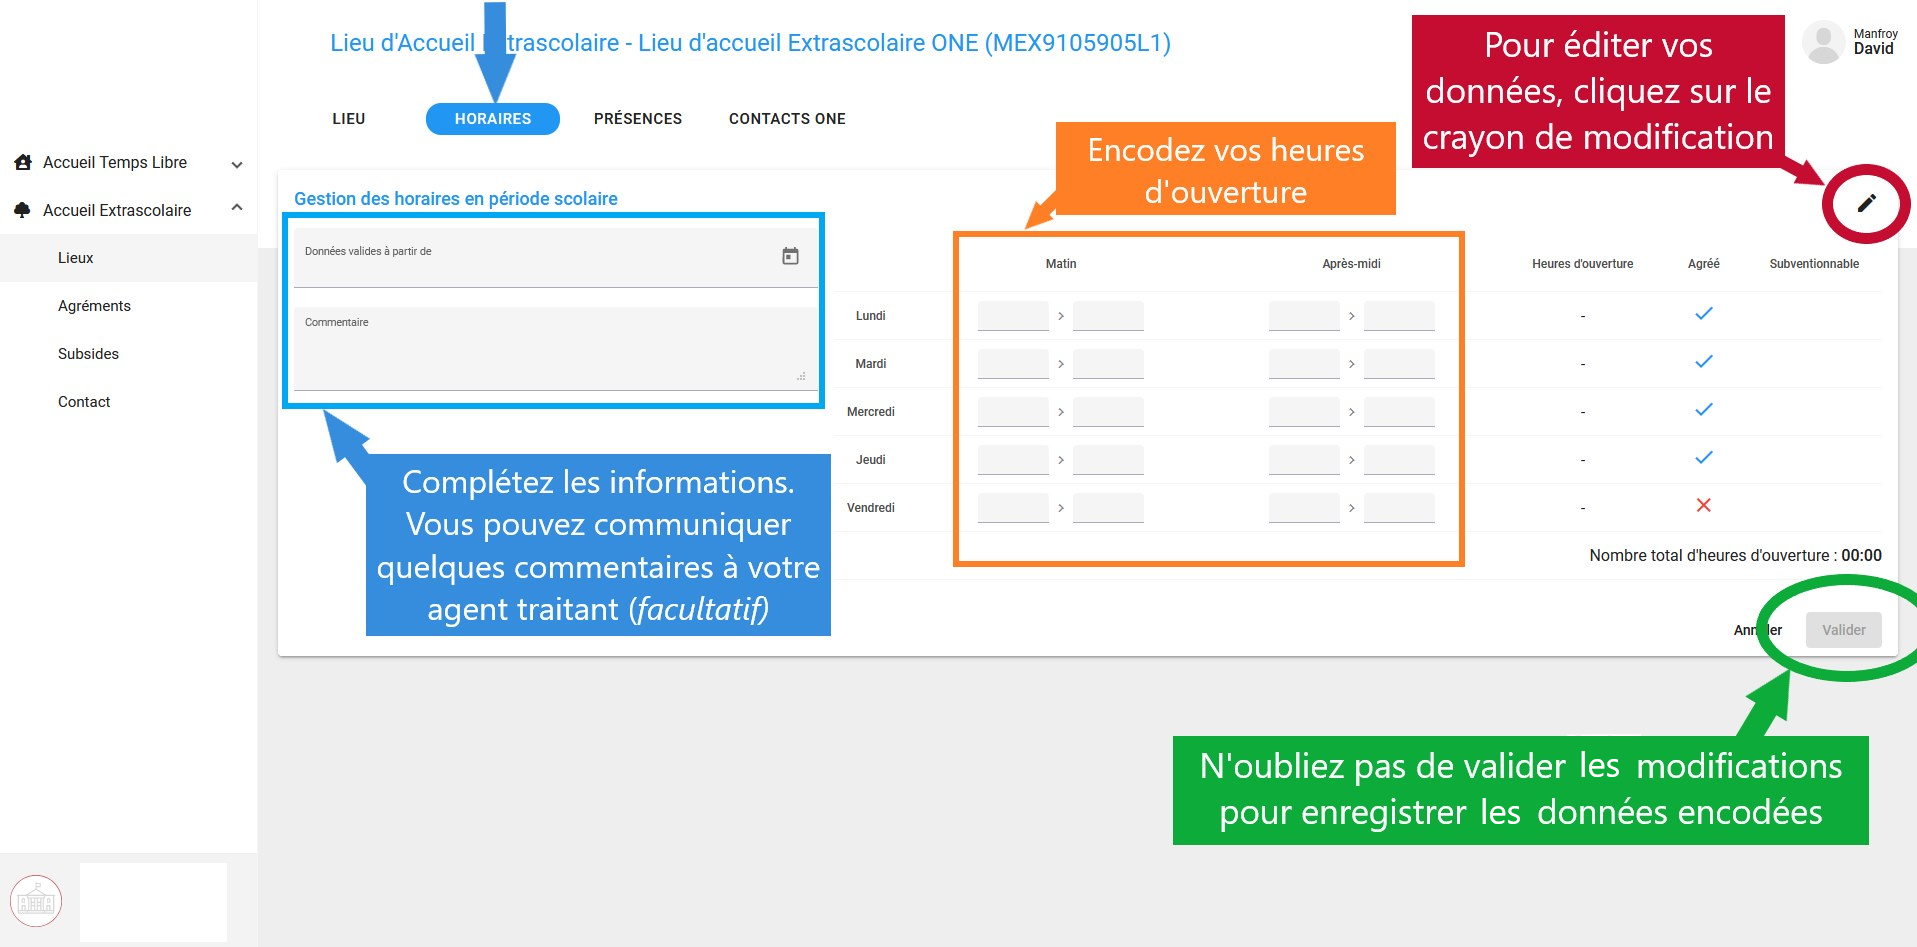
\includegraphics[width=16cm]{Images/aes/horaires.png}}


\subsection{L'onglet encadrement: liste de vos encadrants}

\begin{figure}
    \centering
    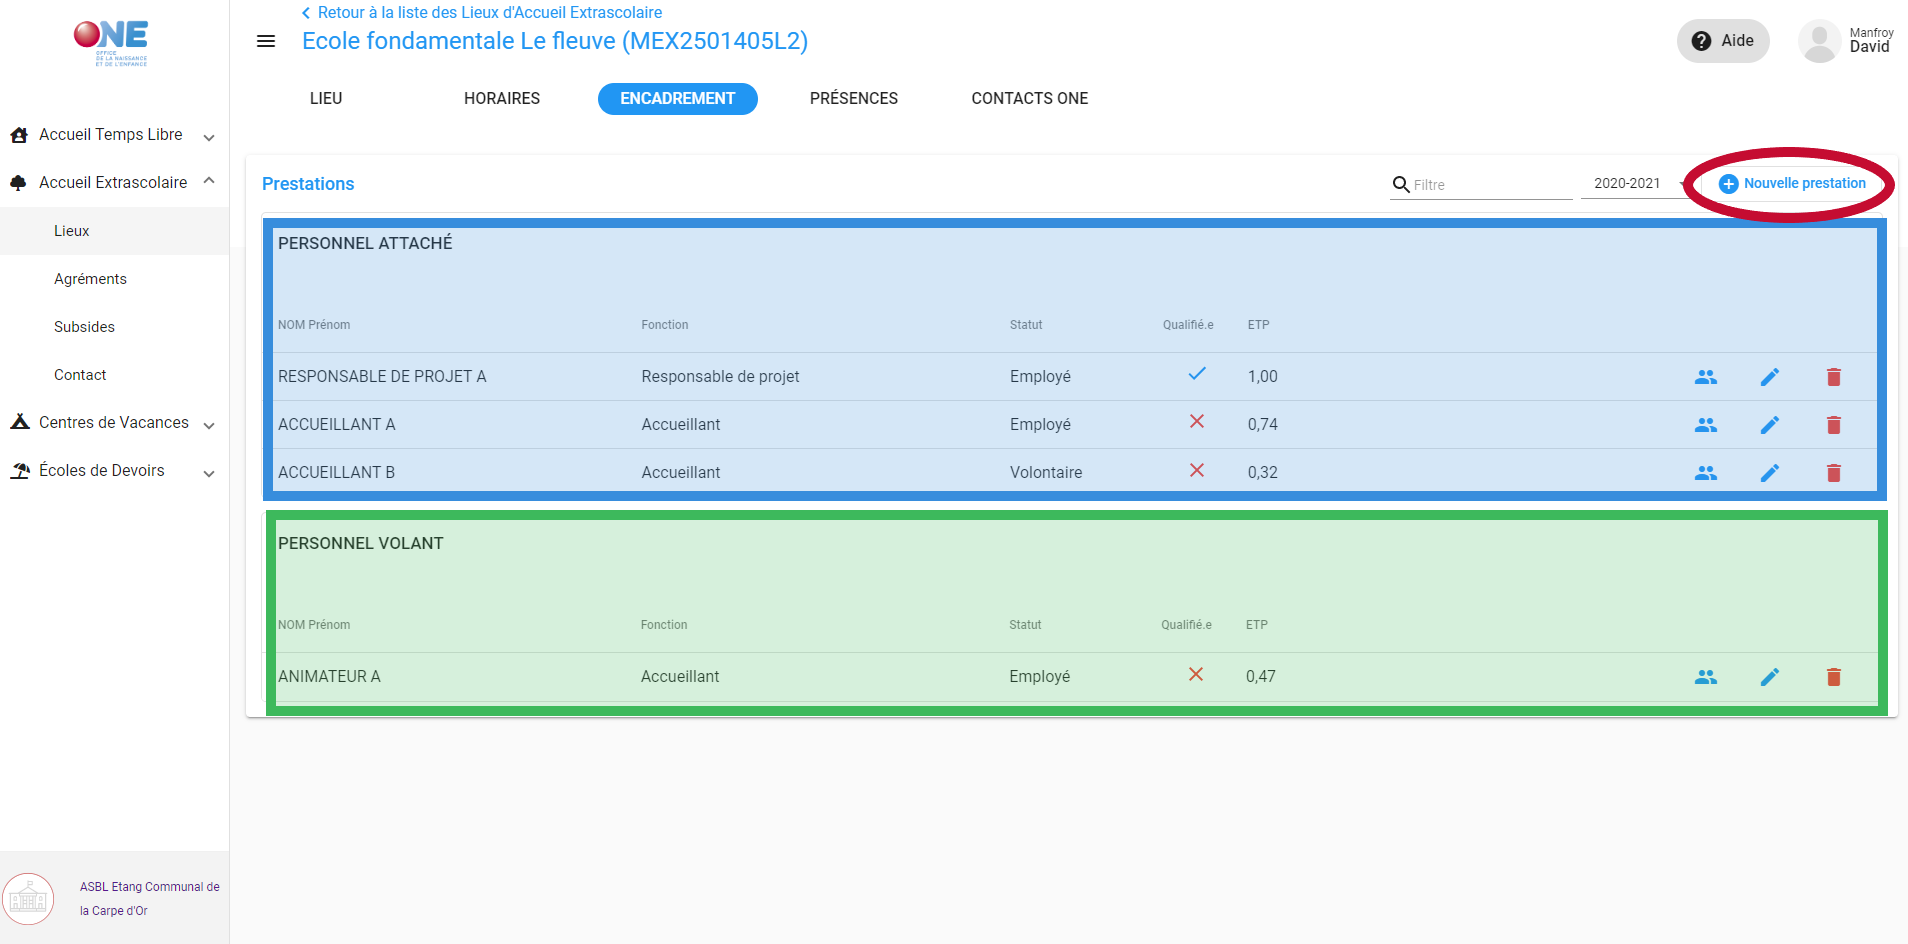
\includegraphics[width=15cm]{Images/aes/encadrement.png}
    \caption{Onglet encadrement: liste du personnel qui preste pour le lieu d'accueil. Vous retrouverez le personnel attaché au lieu d'accueil, ainsi que le personnel volant. Le bouton Nouvelle prestation permet d'ajouter un membre dans l'équipe d'encadrement.}
    \label{fig:aes_encadrement}
\end{figure}


Cet onglet reprend le personnel d'encadrement qui preste pour votre lieu accueil extrascolaire (fig. \ref{fig:aes_encadrement}). Lorsque vous ajouterez le personnel d'encadrement via le bouton "Nouvelle prestation", vous renseignerez les accueillants et les responsables qui encadrent les enfants. Le personnel peut soit être attaché à (en \textcolor{bleu}{bleu}) un (ou plusieurs) lieu d'accueil en particulier ou être volant (\textcolor{vert}{vert})). Chaque personne peut être attachée à un ou plusieurs lieux d'accueil extrascolaire ou être volant. 

Chaque ligne correspond à une prestation. Le tableau du personnel encodé du lieu vous donne:
\begin{itemize}
    \item Le \textbf{nom et prénom} de la personne;
    \item Sa \textbf{fonction}: accueillant ou responsable de projet;
    \item Son \textbf{statut} contractuel (employé, volontaire, ALE, etc.) ou autre lien conventionnel;
    \item Son état de \textbf{qualification}, vous pouvez voir les qualifications de la personne connues par l'ONE:
        \begin{itemize}
            \item [$\bullet$]\textbf{\textcolor{bleu}{V}}: la personne est qualifiée pour exercer sa fonction d'accueillant ou de responsable de projet. 
            \item [$\bullet$]\textbf{\textcolor{rouge}{X}}: la personne n'est pas qualifiée pour exercer sa fonction d'accueillant ou de responsable de projet. 
            \item [$\bullet$]
\includegraphics[width=0.3cm]{Images/icon/icon_sablier.png}: une demande de qualification est en cours d'analyse auprès de l'ONE. 
            \item [$\bullet$]
\includegraphics[width=0.4cm]{Images/icon/icon_attention.png}: la personne a obtenu sa qualification durant l'année en cours.
\end{itemize}
\vspace*{3mm}

    \item Son \textbf{ETP}: le temps de travail de la personne dans sa fonction d'accueillant ou de responsable de projet.
    \item Des \textbf{boutons d'actions}:
    \begin{itemize}
        \item Voir la personne dans Mon Equipe;
        \item Modifier la prestation de la personne;
        \item Supprimer la prestation: la personne n'apparaîtra plus dans le personnel de votre lieu d'accueil pour l'année de référence choisie.
    \end{itemize}
\end{itemize}



\subsubsection{Ajouter un membre du personnel}
Cliquez sur \ovalbox{+ Nouvelle prestation} en haut à droite. Dans l'encadré \fbox{\textbf{Nouvelle prestation}} (fig. \ref{fig:aes_new_prestation}), vous serez invité à encoder l'encadrant et le contexte de sa prestation (contrat de travail, étudiant, stage ou convention de volontariat par exemple), sa fonction, son statut, son temps de travail et son affectation. 

\begin{figure}[htbp]
    \centering
    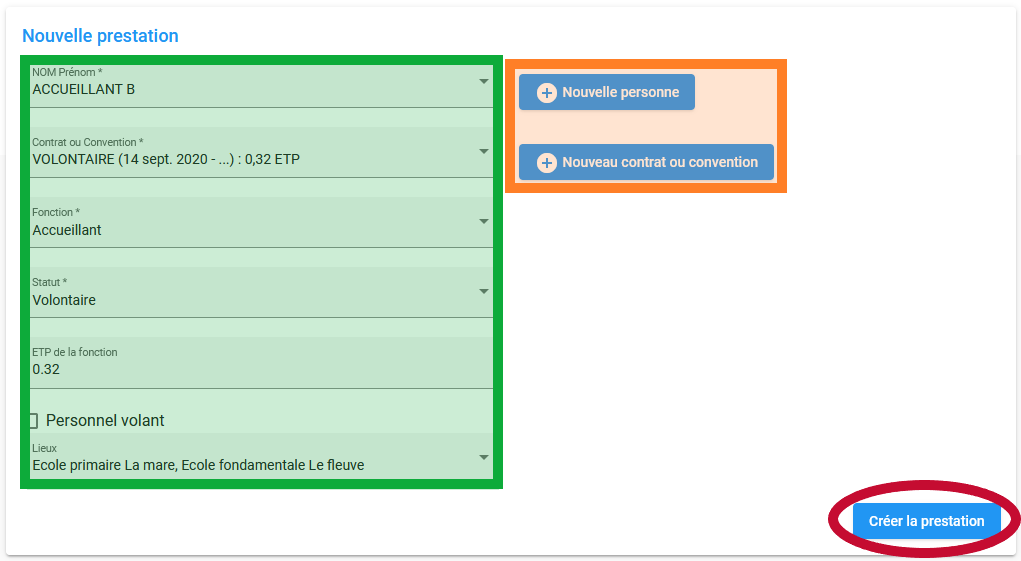
\includegraphics[width=10cm]{Images/aes/add_prestation.png}
    \caption{En cliquant sur Nouvelle prestation, vous êtes invité à encoder les données de la prestation.}
    \label{fig:aes_new_prestation}
\end{figure}


\begin{enumerate}
    \item \textbf{Personne qui a déjà travaillé}: en cliquant sur "\textbf{NOM Prénom}*", vous aurez accès à la liste des personnes qui ont déjà travaillé pour votre pouvoir organisateur dans le secteur de l'accueil extrascolaire;  sélectionnez ensuite la personne dans la liste. 
    \item \textbf{Nouvelle personne}: si par contre, la personne ne figure pas dans la liste, cliquez sur \\\ovalbox{Ajouter une personne}. Vous serez alors dirigé vers "Mon Équipe" pour créer la personne (NISS + Prénom + Nom) et son lien contractuel avec votre Pouvoir organisateur. 
    \begin{info}
     Pour l'encodage d'une nouvelle personne, vous pouvez suivre le point \ref{team_add_person} "Ajouter une personne dans Mon Équipe" du chapitre "Mon Equipe".
    \end{info}
    
    \item En cliquant sur "\textbf{Contrat et convention}", la liste vous donnera l'ensemble des liens (contractuels ou conventionnels) que la personne entretient avec votre pouvoir organisateur. 
    \begin{info}
     Pour l'encodage d'un nouveau contrat, vous pouvez suivre le point \ref{team_add_contract} "Ajouter un contrat/un lien" du chapitre "Mon Equipe".
    \end{info}    

    
    \item Ajoutez la \textbf{fonction}: accueillant ou responsable de projet. 
       
    \item Indiquez le \textbf{statut de la personne}: employé ou volontaire. Ces champs seront pré-remplis en fonction du point 2 (contrat et convention), mais pourront être modifiés. 
    \item Cliquez enfin sur \ovalbox{Créer la prestation}. La personne sera alors ajoutée à la liste des encadrants de votre lieu d'accueil.
\end{enumerate}

\vspace*{4mm}

%\begin{tcolorbox}[title=La personne ou le contrat/convention de celle-ci n'apparaît pas dans la liste de contrat]
%La liste reprend les informations encodées dans "Mon Équipe":
%\begin{itemize}
%    \item \textbf{Pour les personnes}: elles doivent avoir été ajoutées dans Mon Équipe. Elles doivent en outre avoir un contrat en lien avec le secteur Accueil extrascolaire encodées dans mon Équipe.
%    \item \textbf{Pour les contrats/conventions}: la liste ne reprendra que les contrats/conventions dont les dates se chevauchent avec l'année sélectionnée.
%\end{itemize}
%\end{tcolorbox}




%\subsubsection{Envoyer une demande de qualifications}
%\begin{itemize}
%    \item Cliquez sur le petit oeil (consulter la personne dans Mon Équipe). Vous serez dirigé vers la fiche de cette personne et vous pourrez demander une qualification d'accueillant AES et de Responsable de projet AES.
%        \begin{conseil}
%        Suivez le point \ref{sec:qualif_person} de ce Guide pour faire une demande de qualification (Mon Équipe). 
%        \end{conseil}
%    \item Une fois la demande de qualification envoyée dans "Mon Equipe", vous pourrez revenir à la gestion de vos encadrants en cliquant sur le petit encadré jaune "Retourner vers la liste des prestations" situé en bas à droite de votre écran. 
%\end{itemize}



\subsection{L'onglet présences: encodage des présences journalières}
En cliquant sur l'onglet \ovalbox{Présences}, le Portail Pro va ouvrir le tableau de présences journalières des enfants (fig. \ref{fig:aes_présences}). 

Certaines cases journées peuvent apparaître en rouge (non agréées, congés, etc.). Dans ce cas, aucune présence n'est requise. 

Dans \textbf{fréquentation}, Cliquez sur le crayon de modification et complétez le nombre d'enfants inscrits et ayant fréquentés le lieu d'accueil. fréquentation d'enfants de ceux issus de la maternelle et de ceux issus du primaire (en \textcolor{orange}{orange}). Si vous n'accueillez aucun enfant pour l'une ou l'autre section, vous devez encoder "0" (zéro). Si vous ne pouvez pas encoder (case bloquée), vérifiez le type d'accueil dans l'onglet \ovalbox{Lieu}, cadre caractéristiques (cf. point \ref{ssec:aes_lieu}). 

Sélectionnez le trimestre, encodez ensuite les \textbf{présences} des enfants (en {jaune}). Les données sont automatiquement sauvegardées. Un champ commentaire (\textit{facultatif}) est disponible en descendant sous le tableau (en \textcolor{bleu}{bleu} dans la fig.). 




\begin{figure}[htbp]
    \centering
    \includegraphics[width=15cm]{Images/aes/présence2.png}
    \caption{Onglet Présences: encodage de vos présences de vos fréquentations et présences d'enfants. Vous pouvez envoyer une demande de subvention lorsque les données ont été complétées.}
    \label{fig:aes_présences}
\end{figure}
%\centerline{\includegraphics[width=16cm]{Images/aes/présences.png}}


\section{Envoyer une demande de subsides à l'ONE}
Une fois les données de présences encodées pour vos lieux d'accueil, vous pourrez envoyer une demande de subsides prévisionnels à l'ONE. Sous le tableau de présences, vous avez un récapitulatif des données de présences, le montant du subsides prévisionnels et une action \ovalbox{Envoyer} (en \textcolor{vert}{vert} dans la fig. \ref{fig:aes_présences}). 


\begin{remarque}
En cliquant sur le bouton Envoyer, toutes les données de présences seront figées. Pour réaliser une modification, prenez contact avec votre gestionnaire de dossier subsides qui changera le statut de la demande en "renvoyée au PO". Les données seront à nouveau éditables. Une fois vos données de présences corrigées, n'oubliez pas de renvoyer la demande. 
\end{remarque}

%\centerline{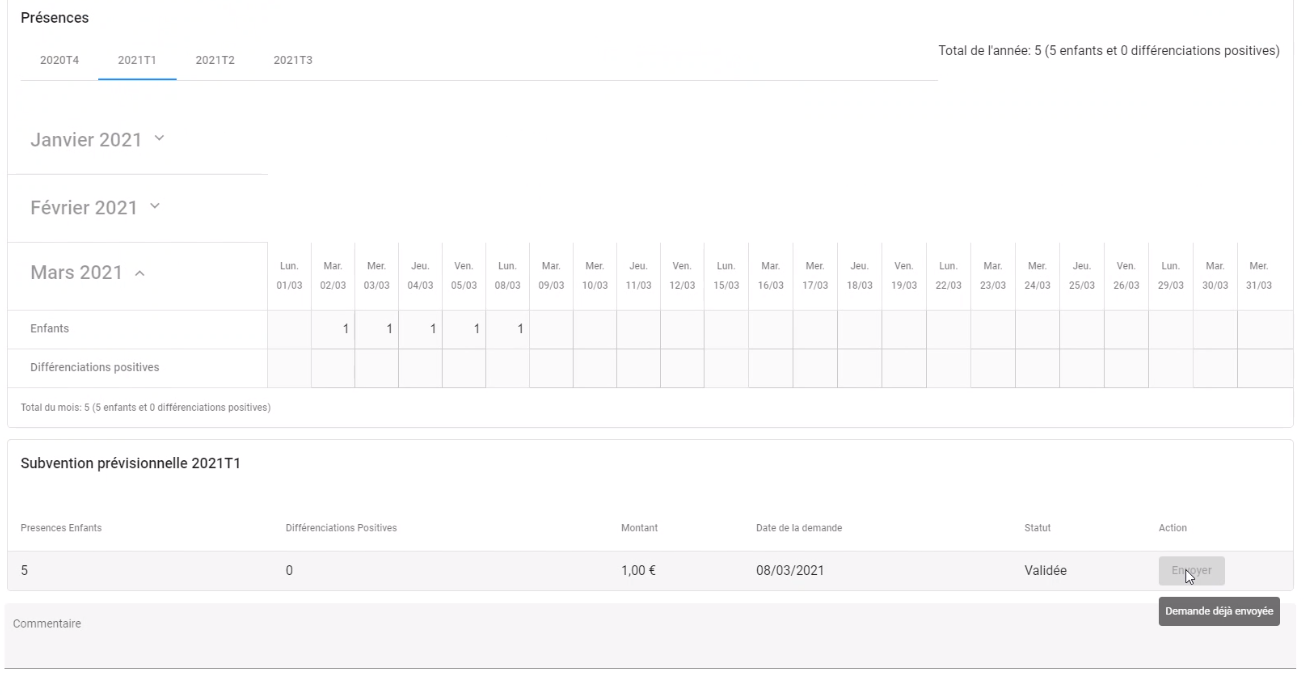
\includegraphics[width=18cm]{Images/aes/aes-ds-envoie.png}}

\section{Agréments}
Dans le volet de navigation, en cliquant sur \ovalbox{Agréments}, vous retrouvez la liste des communes sur le territoire où se déroulent le(s) accueil(s) que vous organisez.
Cette liste mentionne également, si la commune dispose d’un \textbf{programme CLE agréé} ou non, la \textbf{période d’agrément} pour chaque commune et le \textbf{nombre de vos lieux par commune}.

\begin{remarque}
La procédure de renouvellement d’agrément des programmes CLE étant relativement longue, la décision intervient parfois quelques mois après l’échéance du cycle précèdent. Dès lors, ne vous inquiétez pas si la date de fin d’agrément renseignée à l’écran est dépassée.
\end{remarque}